\documentclass[11pt,xcolor={dvipsnames},aspectratio=159,hyperref={pdftex,pdfpagemode=UseNone,hidelinks,pdfdisplaydoctitle=true},usepdftitle=false]{beamer}
\usepackage{presentation}[aspectratio=169]
\usepackage{math}
\usepackage{mathtools}
\usepackage{amsmath}
\usepackage{mleftright}

% Enter title of presentation PDF:
\hypersetup{pdftitle={Aggregate Shocks and Debt Management I}}
% Enter link to PDF file with figures:


\begin{document}
% Enter presentation title:
\title{Aggregate Shocks and Debt Management II}
\subtitle{Fiscal and Monetary Policy 2024}
% Enter presentation information:

% Enter presentation authors:
\author{Piotr Żoch}%
% Enter presentation location and date (optional; comment line if not needed):
\frame{\titlepage}

% Fill out content of presentation:
\begin{frame}{Plan}
    \begin{itemize}
    \item We look at how the U.S. financed its wars over the last 200 years.
    \item We confront these patterns with the predictions of two theories: Barro (1979) and Lucas and Stokey (1983).
    \item We follow the chapter of the Handbook of Historical Economics by Hall and Sargent (2021) -- but we omit many interesting institutional details.
    \end{itemize}
\end{frame}



\begin{frame}
    \heading{Two theories}
\end{frame}

\begin{frame}{Two theories}
\begin{itemize}
\item Recall the two theories we discussed earlier:
\begin{itemize}
\item Barro (1979): incomplete markets
\item Lucas and Stokey (1983): complete markets
\end{itemize}
\item These two theories have different recommendations regarding the optimal mix of taxes and debt to finance wars.
\item We will focus on a simplified version of Lucas and Stokey (1983): assume the same reduced form objective function as in the previous lecture.  
\end{itemize}
\end{frame}


\begin{frame}{Two theories}
    \begin{itemize}
    \item The \al{only} difference is the budget constraint.
    \item In the \alb{Barro (1979) case} the government can only use \al{one-period debt}: 
    \begin{align*}
     \tau_t + a_t = \frac{1}{1+r} a_{t+1} + g_t, 
    \end{align*}     where $a_t$ is a risk free claim on time $t$ goods that the
    government purchased at time $t-1$; debt is $-a_t$.
    \item In the simplified version of \alr{Lucas and Stokey (1983) case} the government can use \al{state-contingent debt}:
    \begin{align*}
        \tau_t + a_{t-1}\bp{s_t} = \int q_t\bp{s_{t+1} \mid s_t } a_{t}\bp{s_{t+1}} ds_{t+1} + g_t, 
       \end{align*} 
    
    where $a_{t-1}\bp{s_t}$ is Arrow security that pays in state $s_t$ and $q_t\bp{\cdot}$ are prices. 
    \end{itemize}
    \end{frame}

\begin{frame}{Two theories}
    \begin{itemize}
        \item Let $PVG_t$ be the expected present value of future government expenditures: 
        \begin{align*}
            PVG_t = \E \bs{\sum_{j=0}^\infty \bp{\frac{1}{1+r}}^j g_{t+j}\mid s_t } = H\bp{s_t}.
        \end{align*}

        \item $H$ satisfies the functional equation
        \begin{align*}
            H\bp{s_t} & = G\bp{s_t} + \frac{1}{1+r} \int H\bp{s_{t+1}}  \phi\bp{s_{t+1}\mid s_t } ds_{t+1} \\
            & = G\bp{s_t} + \frac{1}{1+r} \E \bs{H\bp{s_{t+1}} \mid s_t }.
        \end{align*}
    \end{itemize}
\end{frame}


\begin{frame}{Two theories}
    \begin{itemize}
    \item In Barro (1979) the optimal plan is 
    \begin{align*}  
    \tau_t = \frac{r}{1+r}\bs{H\bp{s_t}+a_t}
    \end{align*}
    and has the implication that taxes are a random walk
    \begin{align*}  
        \E_{t}\bs{\tau_{t+1}} = \tau_t.
        \end{align*}
        \item Government assets are also a random walk.
    \end{itemize}
    \end{frame}

\begin{frame}{Two theories}
    \begin{itemize}
        \item This simplified version of Lucas and Stokey (1983) has the optimal plan that 
    \begin{align*}
       \tau_t = \tau_0.
        \end{align*}
    \item The state-contingent asset-purchasing strategy supports this tax collection policy:
    \begin{align*}
        a_{t-1}\bp{s_t} = H\bp{s_t} - \frac{1+r}{r} \tau_0.
    \end{align*} 
\end{itemize}
\end{frame}


\begin{frame}{Two theories}
    \begin{itemize}
    \item To facilitate comparison we assume 
    \begin{align*}  
    q\bp{s_{t+1} \mid s_t } = \frac{1}{1+r} \phi\bp{s_{t+1} \mid s_t }.
    \end{align*}
    \item This results in the budget constraint for the Lucas and Stokey (1983) case: 
    \begin{align*}
        \tau_t + a_{t-1}\bp{s_t} = \frac{1}{1+r} \E \bs{a_{t+1} \mid s_t} + g_t, 
    \end{align*}
    where we define $\E \bs{a_{t+1} \mid s_t } = \int a_{t}\bp{s_{t+1}} \phi\bp{s_{t+1} \mid s_t } ds_{t+1}$.
    \end{itemize}
    \end{frame}
    
    
    \begin{frame}{Ex-post returns}
        \begin{itemize}
        \item Useful to distinguish between \al{ex-ante} and \al{ex-post} returns.
        \item Ex-post return on a portfolio of Arrow securities is 
        \begin{align*}
            R_t \bp{s_{t+1}\mid s_t}=\frac{a_t\bp{s_{t+1}}}{\E \bs{a_{t+1} \mid s_t }}  
        \end{align*}
        \item The conditional expectation of the return on the government portfolio (ex-ante) is then
        \begin{align*}
            \E\bs{R_t \bp{s_{t+1}\mid s_t}\mid s_t} = 1+r
        \end{align*}    
    \end{itemize}
        \end{frame}

        

\begin{frame}{Two theories}
    \begin{figure}
        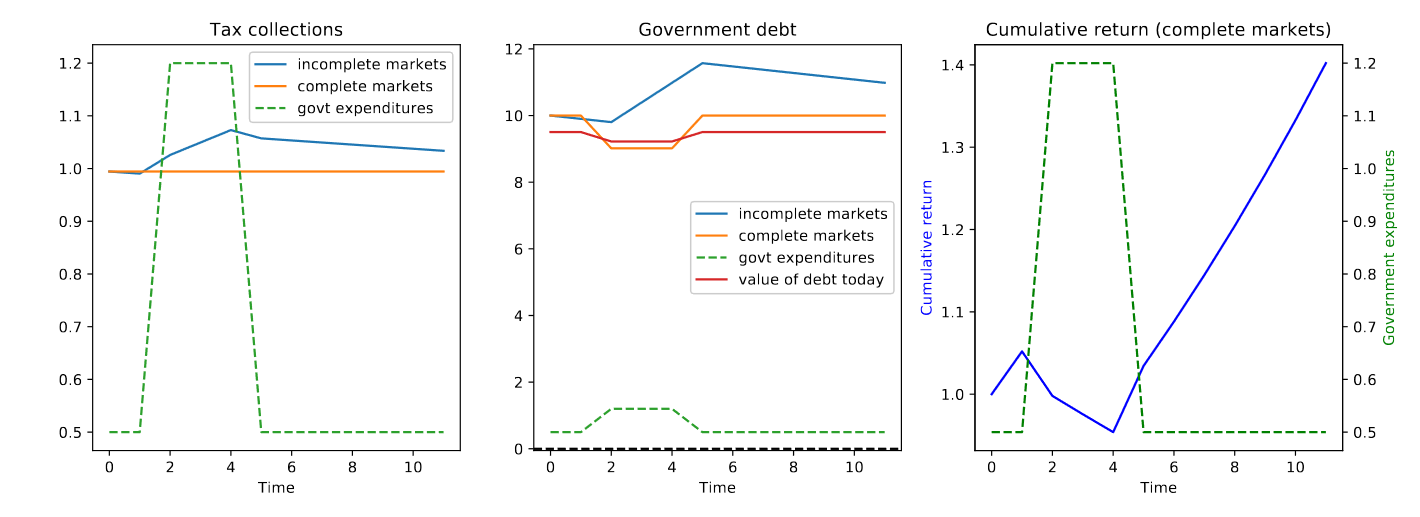
\includegraphics[width=1\textwidth]{comparison.png}
        \caption{Tax and debt policy in complete and incomplete markets.} 
    \end{figure}
\end{frame}


\begin{frame}
    \heading{Government budget constraint}
\end{frame}


\begin{frame}{Government budget constraint}
    \begin{itemize}
        \item We need to map the model into the data. 
        \item Let $B_{t-1} = \sum_{j=1}^{n} B_{t-1}^j$ be the total nominal value of interest bearing government
        debt at $t-1$, where $B_{t-1}^j$ is the nominal value of zero coupon bonds of maturity $j$ at $t-1$.
        \item The government budget constraint at time $t$ is 
        \begin{align*}
            B_t = B_{t-1} + r_{t-1,t} B_{t-1} + G_t - T_t - \bp{M_t - M_{t-1}},
        \end{align*}
        where $M_t$ is the nominal money supply and $r_{t-1,t}$ is implicitly defined by 
        $$ r_{t,t-1} B_{t-1} = \sum_{j=1}^{n} r^j_{t-1,t} B_{t-1}^j.   $$
        \item All variables above are \al{nominal}.
     
        
    \end{itemize}
\end{frame}

\begin{frame}{Government budget constraint}
    \begin{itemize}
        \item Hall and Sargent make two adjustments to the U.S. Treasury's
        record of total public debt outstanding:
        \begin{enumerate}
            \item net out holdings by the Federal Reserve and
            Government Agencies and Trust Funds;
            \item  measure Treasury debt by its market value
            rather than its par value.
        \end{enumerate}
     
        
    \end{itemize}
\end{frame}


\begin{frame}{Debt ownership}
    \begin{figure}
        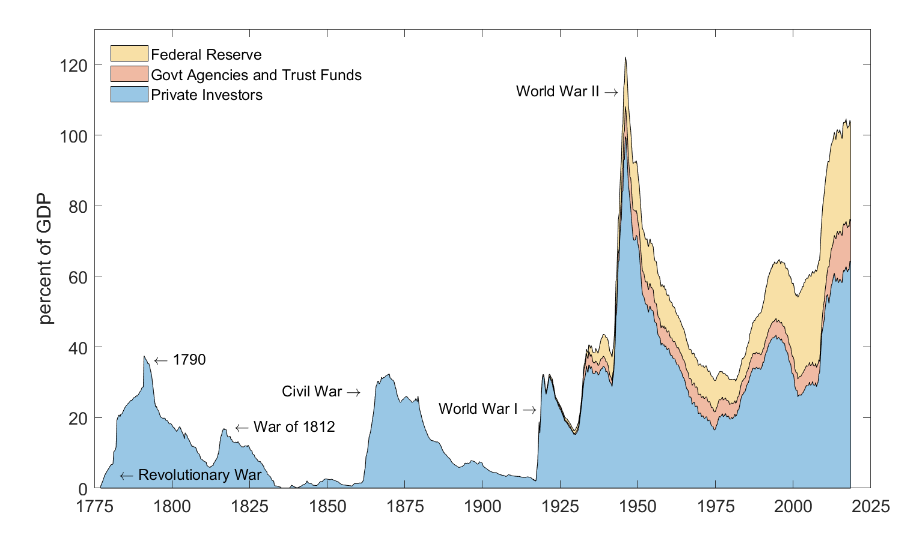
\includegraphics[width=0.8\textwidth]{debt_owner.png}
    \end{figure}
\end{frame}

\begin{frame}{Debt value}
    \begin{figure}
        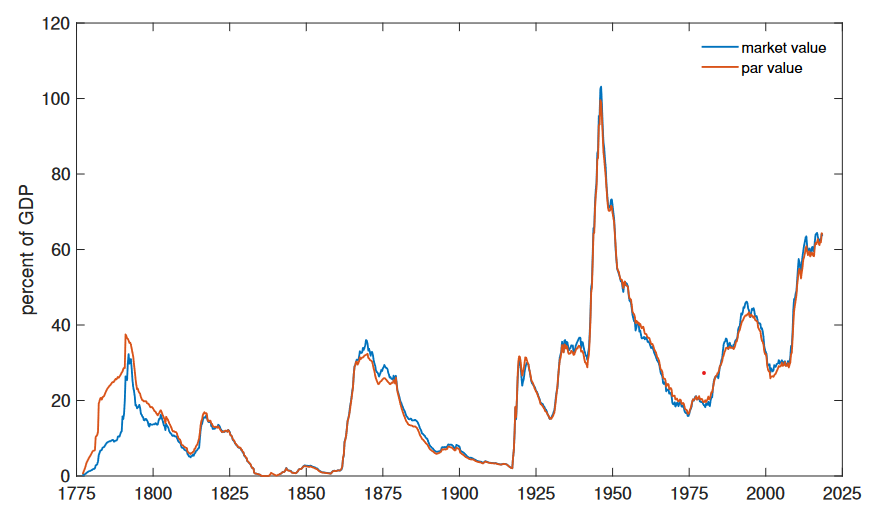
\includegraphics[width=0.8\textwidth]{debt_value.png}
    \end{figure}
\end{frame}


\begin{frame}{Government budget constraint}
\begin{itemize}
\item We can rewrite the budget constraint as 
\begin{align*}
    \frac{G_t}{Y_t} + r_{t-1,t} \frac{B_{t-1}}{Y_{t-1}} &= \frac{T_t}{Y_t}  + \bp{\frac{B_t}{Y_t} -\frac{B_{t-1}}{Y_{t-1}} } + \frac{M_t - M_{t-1}}{Y_t} \\
    & + g_{t-1,t} \frac{B_{t-1}}{Y_{t-1}}  + \pi_{t-1,t} \frac{B_{t-1}}{Y_{t-1}} \\
    & +  r_{t-1,t}\bp{g_{t-1,t}+\pi_{t-1,t}} \frac{B_{t-1}}{Y_{t-1}} 
\end{align*}
where $g_{t-1,t}$ denotes the growth rate of real GDP, and $\pi_{t-1,t}$ denotes the inflation rate.
\item The first three terms on the right
side record sources of government revenue as shares of GDP: taxes, new borrowing and money
creation. 
\item The next two terms record the diminution of the debt/GDP ratio due to real GDP
growth and inflation.
\end{itemize}
\end{frame}
%
\begin{frame}{Government budget constraint}
    \begin{itemize}
    \item  A "peacetime baseline" version of the constraint
    \begin{align*}
        \bp{\frac{G}{Y}}^{\text{base}} + \bp{r_{-1,0} \frac{B_{-1}}{Y_{-1}}}^{\text{base}} &= \bp{\frac{T}{Y}}^{\text{base}}  + \bp{\frac{B}{Y} -\frac{B_{-1}}{Y_{-1}} }^{\text{base}} \\
        & + \bp{\frac{M - M_{-1}}{Y}}^{\text{base}} \\
        & + \bp{g_{-1,0} \frac{B_{-1}}{Y_{-1}}}^{\text{base}}  + \bp{\pi_{-1,0} \frac{B_{-1}}{Y_{-1}}}^{\text{base}} \\
        & +  \bp{r_{-1,t}\bp{g_{-1,0}+\pi_{-1,0}} \frac{B_{-1}}{Y_{-1}}}^{\text{base}} 
    \end{align*}
    
    \end{itemize}
    \end{frame}

\begin{frame}{Government budget constraint}
    \begin{itemize}
    \item In each period we can calculate deviation of "wartime" budget constraint from the "peacetime baseline".
    \item Hall and Sargent sum from the beginning of the war to the end of the war to get the total wartime deviation.
    \begin{align*}
        \footnotesize
        \sum_{t=T_1}^{T_2} \bs{\frac{G_t}{Y_t} - \bp{\frac{G}{Y}}^{\text{base}}} + \sum_{t=T_1}^{T_2}\bs{r_{t-1,t} \frac{B_{t-1}}{Y_{t-1}}-\bp{r_{-1,0} \frac{B_{-1}}{Y_{-1}}}^{\text{base}}} & \\
        = \sum_{t=T_1}^{T_2} \bs{\frac{T_t}{Y_t}-\bp{\frac{T}{Y}}^{\text{base}}} + \sum_{t=T_1}^{T_2} \bs{\bp{\frac{B_t}{Y_t} -\frac{B_{t-1}}{Y_{t-1}} }-\bp{\frac{B}{Y} -\frac{B_{-1}}{Y_{-1}} }^{\text{base}} }  \\
        + \sum_{t=T_1}^{T_2} \bs{\frac{M_t - M_{t-1}}{Y_t}-\bp{\frac{M - M_{-1}}{Y}}^{\text{base}}} 
        +  \cdots
    \end{align*}
    
    \end{itemize}
    \end{frame}
%
\begin{frame}
    \begin{figure}
        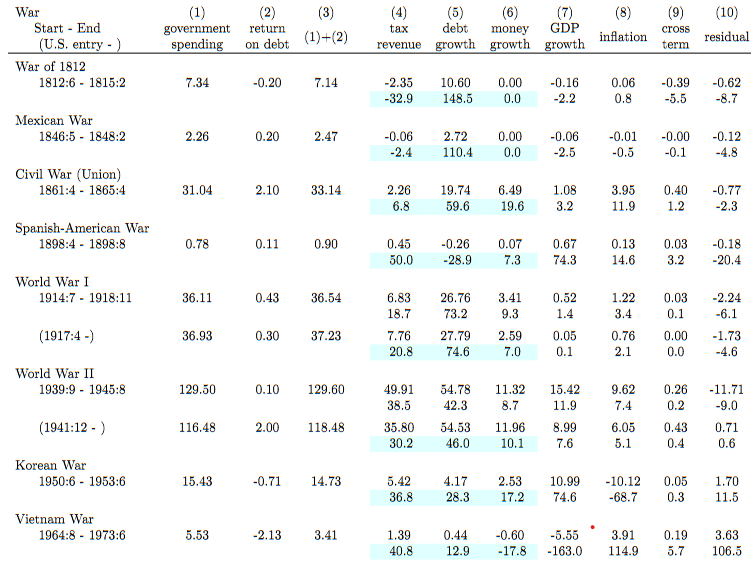
\includegraphics[width=0.8\textwidth]{table1.png}
    \end{figure}
\end{frame}

\begin{frame}{Optimal response}
    \begin{itemize}
    \item Suppose $r=0.06$, the net real interest rate in our model is 6\%. 
    \item Barro (1979) implies that a purely transitory increse in $g_t$ should be financed in 6\% by taxes and in 94\% by debt. 
    \item We see it for the Civil War only.
    \item Caveat: were these increases in government purchases really transitory?
    \end{itemize}
    \end{frame}

    \begin{frame}{Receipts and expenditures}
        \begin{figure}
            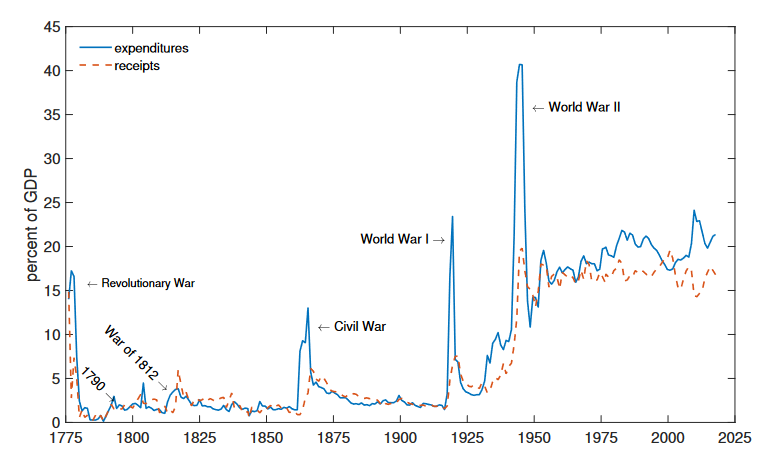
\includegraphics[width=0.8\textwidth]{receiptsexpenditures.png}
        \end{figure}
    \end{frame}


    \begin{frame}{Optimal response}
        \begin{itemize}
        \item  Lucas and Stokey (1983) implies that unexpected increases in government spending should be absorbed by wartime decreases in returns to government creditors.
        \item  With the exception of the Mexican War and the Korean War, the contribution of inflation is greater than the contribution of the nominal return on the debt.
        \item Negative wartime real returns.
        \end{itemize}
        \end{frame}





\begin{frame}
    \begin{figure}
        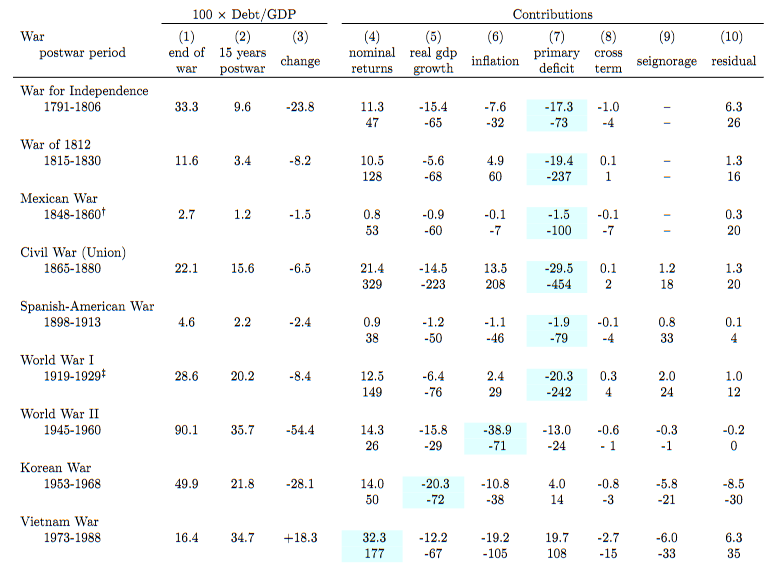
\includegraphics[width=0.8\textwidth]{table2.png}
    \end{figure}
\end{frame}

\begin{frame}{Prices}
    \begin{figure}
        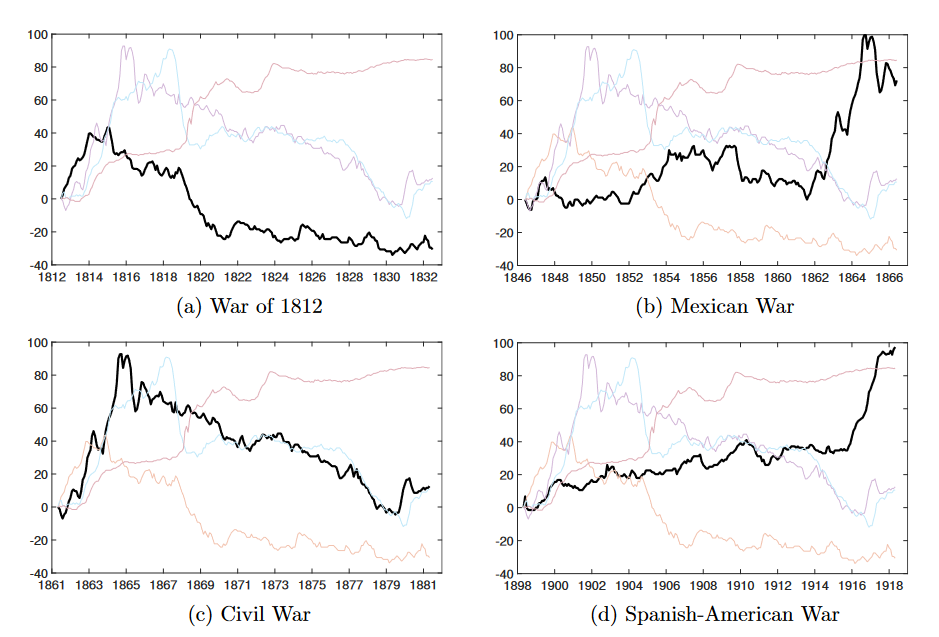
\includegraphics[width=0.8\textwidth]{prices1.png}
    \end{figure}
\end{frame}

\begin{frame}{Prices}
    \begin{figure}
        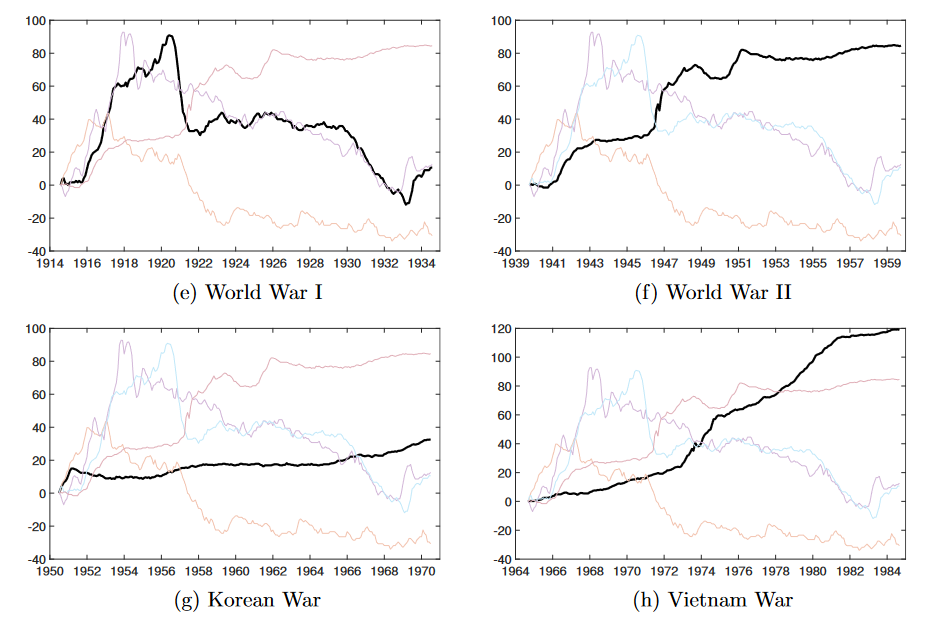
\includegraphics[width=0.8\textwidth]{prices2.png}
    \end{figure}
\end{frame}

\begin{frame}{Returns}
    \begin{figure}
        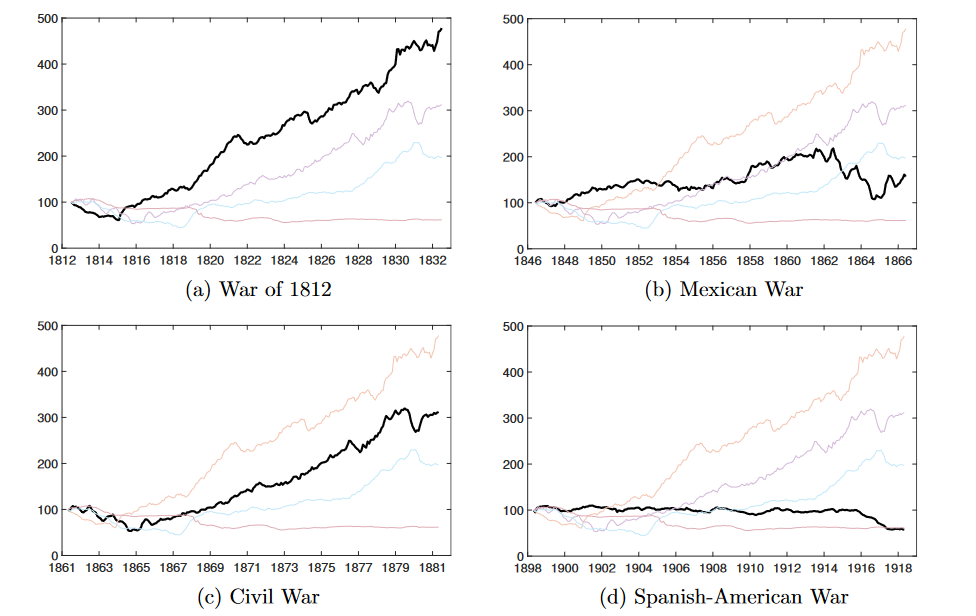
\includegraphics[width=0.8\textwidth]{portfolio1.png}
    \end{figure}
\end{frame}

\begin{frame}{Returns}
    \begin{figure}
        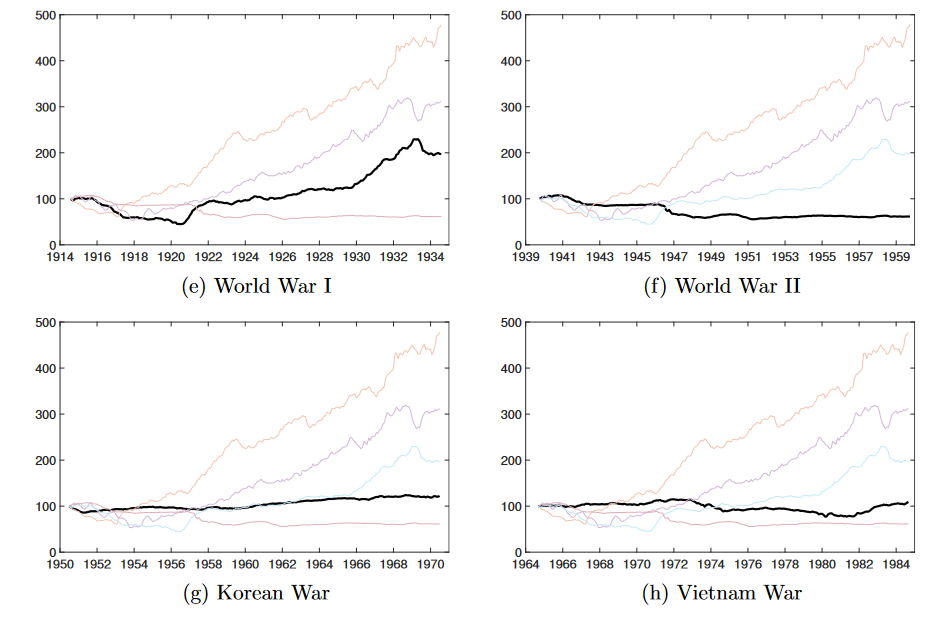
\includegraphics[width=0.8\textwidth]{portfolio2.png}

    \end{figure}
\end{frame}

\begin{frame}{Conclusions}
    
 \begin{itemize}
\item  Evidence of Barro tax smoothing in most wars, but only during the Civil War the split between taxes and debt that the model recommends for a purely temporary expenditure
surge. 
\item Negative wartime bond returns followed by positive postwar returns in the
War of 1812, the Civil War, World War I and the Korean War as prescribed by the Lucas-Stokey
model 
\item However, this model directs that bondholders should receive an immediate capital loss
at the outbreak of a war. This happens  only in the Korean War. 
\item The U.S. had little debt at the outbreak of most wars, the Lucas-Stokey
action would not help the government's financial situation.
 \end{itemize}

\end{frame}
\end{document}